% Generated by src/report.py. Edit that template for lasting changes.
% Basics: \section{...} creates headings; \[ ... \] displays mathematics.
\documentclass[11pt,a4paper]{article}
\usepackage[T1]{fontenc}
\usepackage[utf8]{inputenc}
\usepackage[margin=2.2cm]{geometry}
\usepackage{amsmath,booktabs,graphicx}
\usepackage{xcolor,fancyhdr,microtype,lmodern}
\usepackage[hidelinks]{hyperref}
\definecolor{ink}{HTML}{17354A}
\pagestyle{fancy}\fancyhf{}
\fancyhead[L]{\small\textsc{Stochastic Processes in Finance}}
\fancyhead[R]{\small AAPL and VIX}
\fancyfoot[C]{\small\thepage}
\setlength{\headheight}{14pt}
\setlength{\parindent}{0pt}\setlength{\parskip}{6pt}
\renewcommand{\arraystretch}{1.25}
\title{\color{ink}Stochastic Processes in Finance\\\large An Empirical Comparison of AAPL and VIX}
\author{}\date{}
\begin{document}\maketitle
\begin{abstract}
This study compares a geometric random walk, geometric Brownian motion,
and an exponentiated Ornstein--Uhlenbeck process with observed AAPL stock
prices and the VIX volatility index. Each asset is studied using 504 daily
log returns and 200 simulated paths per model. The comparison considers
return moments, serial dependence, stationarity diagnostics, and drawdown.
The exercise evaluates in-sample descriptive fit; it does not establish
predictive performance or market efficiency.
\end{abstract}

\section{Research objective and hypotheses}
The objective is to assess which empirical features of two contrasting
financial series can be reproduced by simple stochastic processes.
VIX is a volatility index, not a directly investable stock price; applying
price-process models to it is an illustrative statistical exercise.

The original research questions are expressed as four hypotheses:
\begin{enumerate}
\item \textbf{H1: Weak return dependence.} Returns have little serial
correlation. Autocorrelation is examined as a limited diagnostic of the
broader weak-form efficiency question.
\item \textbf{H2: Random-walk approximation.} A geometric random walk
reproduces observed return and risk characteristics reasonably well.
\item \textbf{H3: GBM distributional fit.} Gaussian log-return increments
provide an adequate description of the observed distribution.
\item \textbf{H4: Mean reversion.} Log-price stationarity is consistent
with using a mean-reverting process. An ADF test is a diagnostic, not proof
of OU dynamics.
\end{enumerate}

\clearpage
\section{Data and methodology}
The analysis uses the local snapshots \texttt{Data/Assets/stock.csv} and
\texttt{Data/Assets/index.csv}, originally sourced through yfinance.
Each series contributes its last 505 closing observations, giving 504
log returns, $r_t=\log(S_t/S_{t-1})$. The CSV files contain no date column,
so exact calendar coverage cannot be reconstructed from these inputs.
The report is rebuilt from both snapshots without downloading fresh data.

Each asset uses 200 paths of 504 increments, $\Delta t=1/252$, and random
seed 51 reset separately for reproducibility. Inputs are estimated from
the same sample used for comparison, making this an in-sample study.
Annualized mean and volatility use $m=252\bar r$ and
$\sigma=\sqrt{252}\,\operatorname{std}(r)$, with population standard deviation.

\subsection{Implemented processes}
Let $Z_t$ be independent standard normal draws and $X_t=\log S_t$:
\begin{align*}
\text{RW:}\quad S_{t+1}&=S_t\exp(\sqrt{\Delta t}Z_t),\\
\text{GBM:}\quad S_{t+1}&=S_t\exp\bigl[(m-\sigma^2/2)\Delta t+\sigma\sqrt{\Delta t}Z_t\bigr],\\
\text{Log-OU:}\quad X_{t+1}&=X_t+\theta(\ell-X_t)\Delta t+\sigma\sqrt{\Delta t}Z_t,
\quad S_t=e^{X_t}.
\end{align*}
Here $\ell$ is the sample mean log price and $\theta$ is specified rather
than fitted. The random walk fixes annual log volatility at one.
The GBM code uses the observed mean log return as $m$ and then subtracts
$\sigma^2/2$, so expected annual log return is $m-\sigma^2/2$, rather than $m$.
This implementation detail is retained and must inform interpretation.

\begin{table}[htbp]\centering
\caption{Model inputs. Starting levels retain their original units.}
\begin{tabular}{lrrrrr}\toprule
Asset & $S_0$ & $m$ & $\sigma$ & $\ell$ & $\theta$ \\\midrule
AAPL & 168.05 & 0.2191 & 0.2814 & 5.4276 & 2.5 \\
VIX & 16.03 & 0.0910 & 1.4147 & 2.8723 & 3.0 \\
\bottomrule\end{tabular}\end{table}

\subsection{Measurement conventions}
Simulated return moments use pooled paths. Return ADF tests and
correlations use flattened paths, creating artificial joins between
independent simulations. Simulated price ADF p-values and drawdowns are
averages of per-path statistics; average p-values are not combined tests.
Observed and OU price ADF tests use log prices, whereas RW and GBM use
levels. Pearson kurtosis equals three under normality. Drawdowns are
negative losses relative to preceding peaks.

\clearpage
\section{Results: AAPL}
\begin{table}[htbp]\centering
\caption{AAPL: observed and simulated statistics.}
\resizebox{\linewidth}{!}{\begin{tabular}{lrrrr}\toprule
Metric & AAPL & RW & GBM & Log-OU \\
\midrule
Annualized mean log return & 21.91\% & 0.47\% & 20.13\% & 15.04\% \\
Annualized volatility & 28.14\% & 99.74\% & 28.20\% & 28.23\% \\
Return autocorrelation (lag 1) & 0.05196 & -0.0003034 & -0.00425 & -0.003942 \\
ADF p-value: returns & $<10^{-4}$ & $<10^{-4}$ & $<10^{-4}$ & $<10^{-4}$ \\
ADF p-value: price series & 0.1798 & 0.4088 & 0.5741 & 0.2197 \\
Return skewness & 0.5675 & -0.001577 & -0.005083 & 0.004781 \\
Return kurtosis (Pearson) & 13.77 & 2.994 & 2.973 & 2.998 \\
Maximum drawdown & -33.36\% & -77.41\% & -28.03\% & -28.68\% \\
\bottomrule\end{tabular}}\end{table}
The sample contains 504 observed daily log returns. Its annualized mean log return is 21.91\% and annualized volatility is 28.14\%.

\subsection{Distribution and risk}
Observed Pearson kurtosis is 13.77, versus 2.97--3.00 across the simulated models. Observed skewness is 0.567. Gaussian shocks do not reproduce the observed higher return moments in this run. Observed maximum drawdown is -33.36\%; model drawdowns are path averages and should not be treated as forecasts.

\subsection{Persistence and model fit}
Lag-one return autocorrelation is 0.052. This is a descriptive measure, not a formal test of market efficiency. The ADF test on observed log prices does not reject the unit-root null at the 5\% level. That result alone does not identify an OU process. GBM simulated volatility is 28.20\%, while its annualized mean log return is 20.13\%. The drift convention discussed above explains why the mean need not match the data.

\small RW: geometric random walk; GBM: geometric Brownian motion; Log-OU: exponentiated OU process.\normalsize
\clearpage
\subsection*{AAPL: Price dynamics}
\begin{figure}[!htbp]\centering
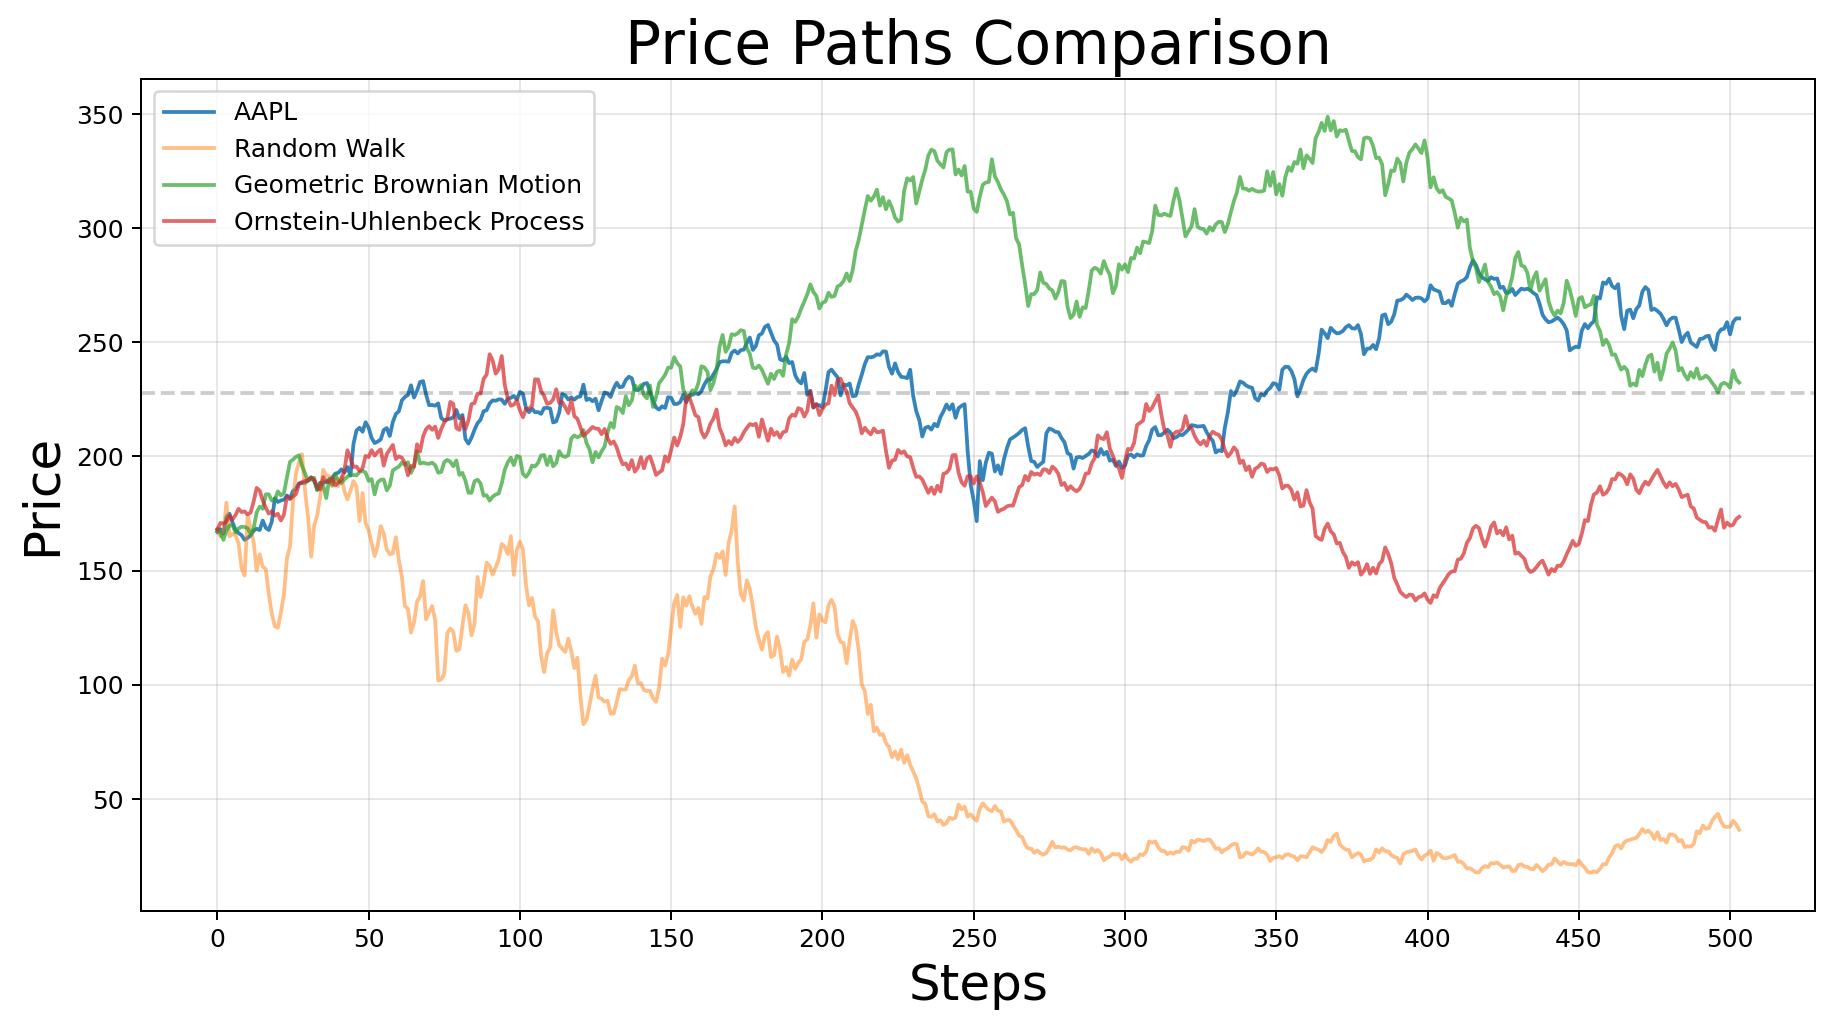
\includegraphics[width=\linewidth,height=0.35\textheight,keepaspectratio]{figures/AAPL/price_paths.png}
\caption{AAPL: Observed series and one illustrative path per model.}
\end{figure}
\begin{figure}[!htbp]\centering
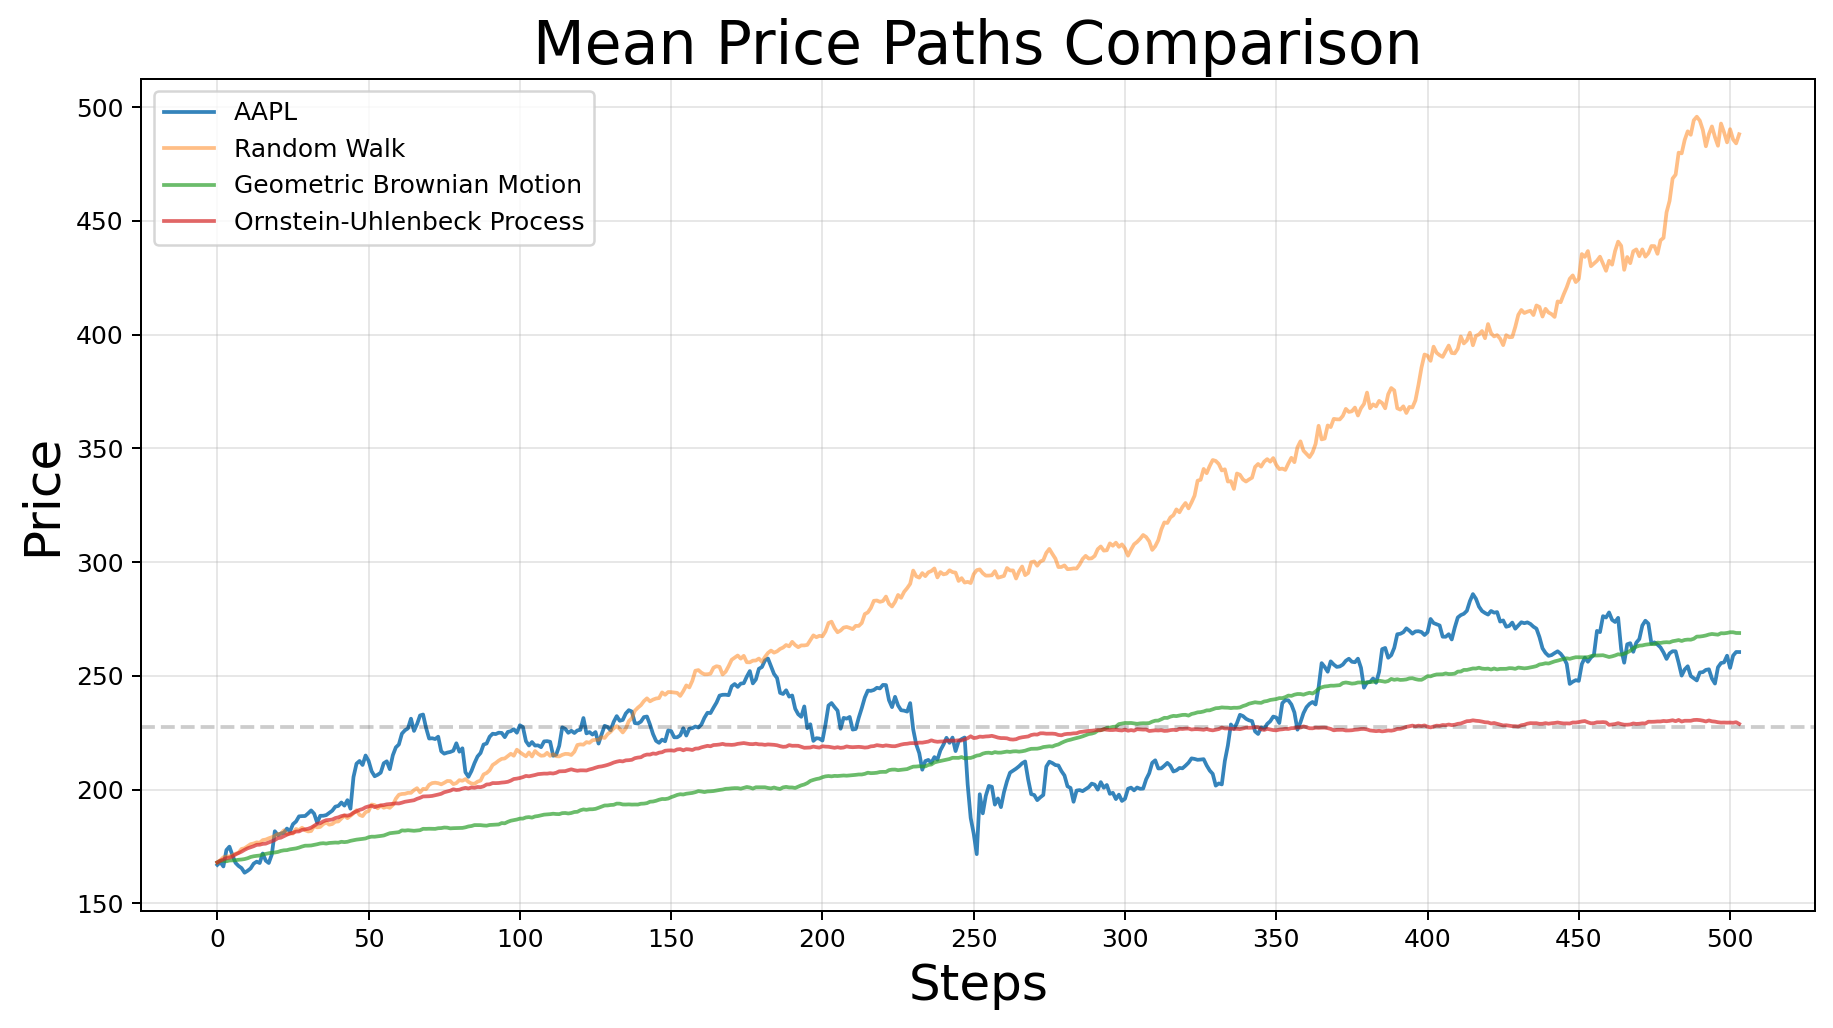
\includegraphics[width=\linewidth,height=0.35\textheight,keepaspectratio]{figures/AAPL/mean_paths.png}
\caption{AAPL: Observed series and ensemble mean of 200 simulated paths.}
\end{figure}
\clearpage
\subsection*{AAPL: Return diagnostics}
\begin{figure}[!htbp]\centering
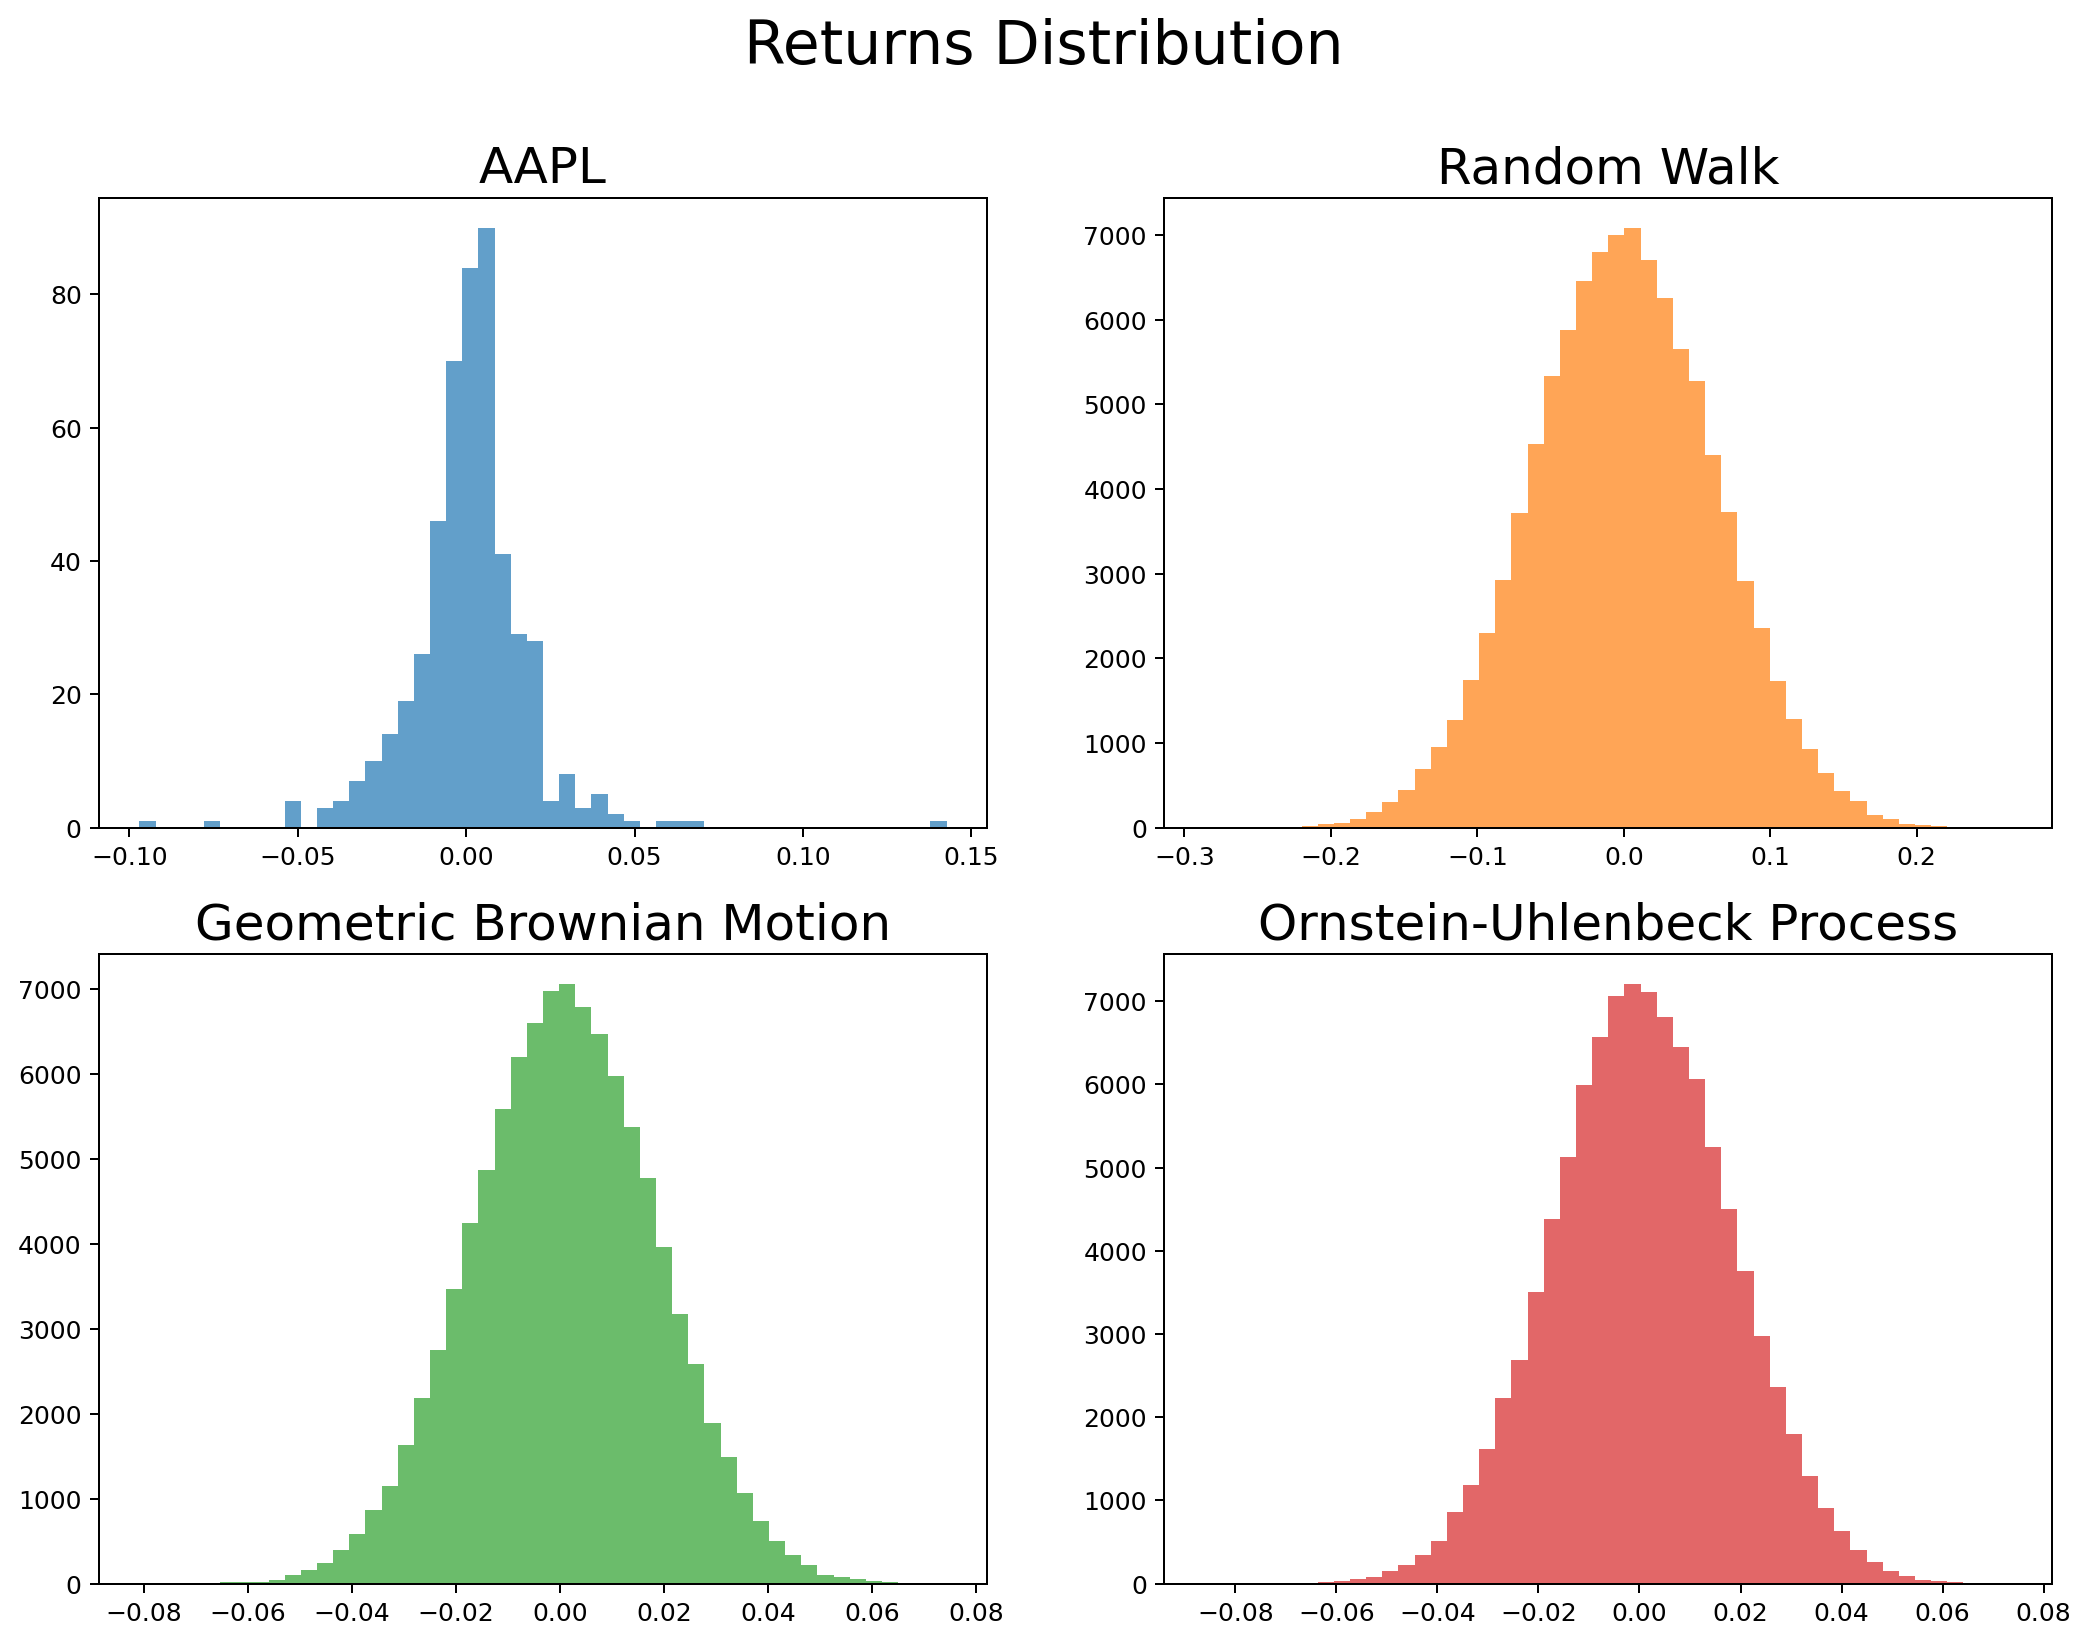
\includegraphics[width=\linewidth,height=0.35\textheight,keepaspectratio]{figures/AAPL/distributions.png}
\caption{AAPL: Observed and simulated log-return distributions; counts use different sample sizes.}
\end{figure}
\begin{figure}[!htbp]\centering
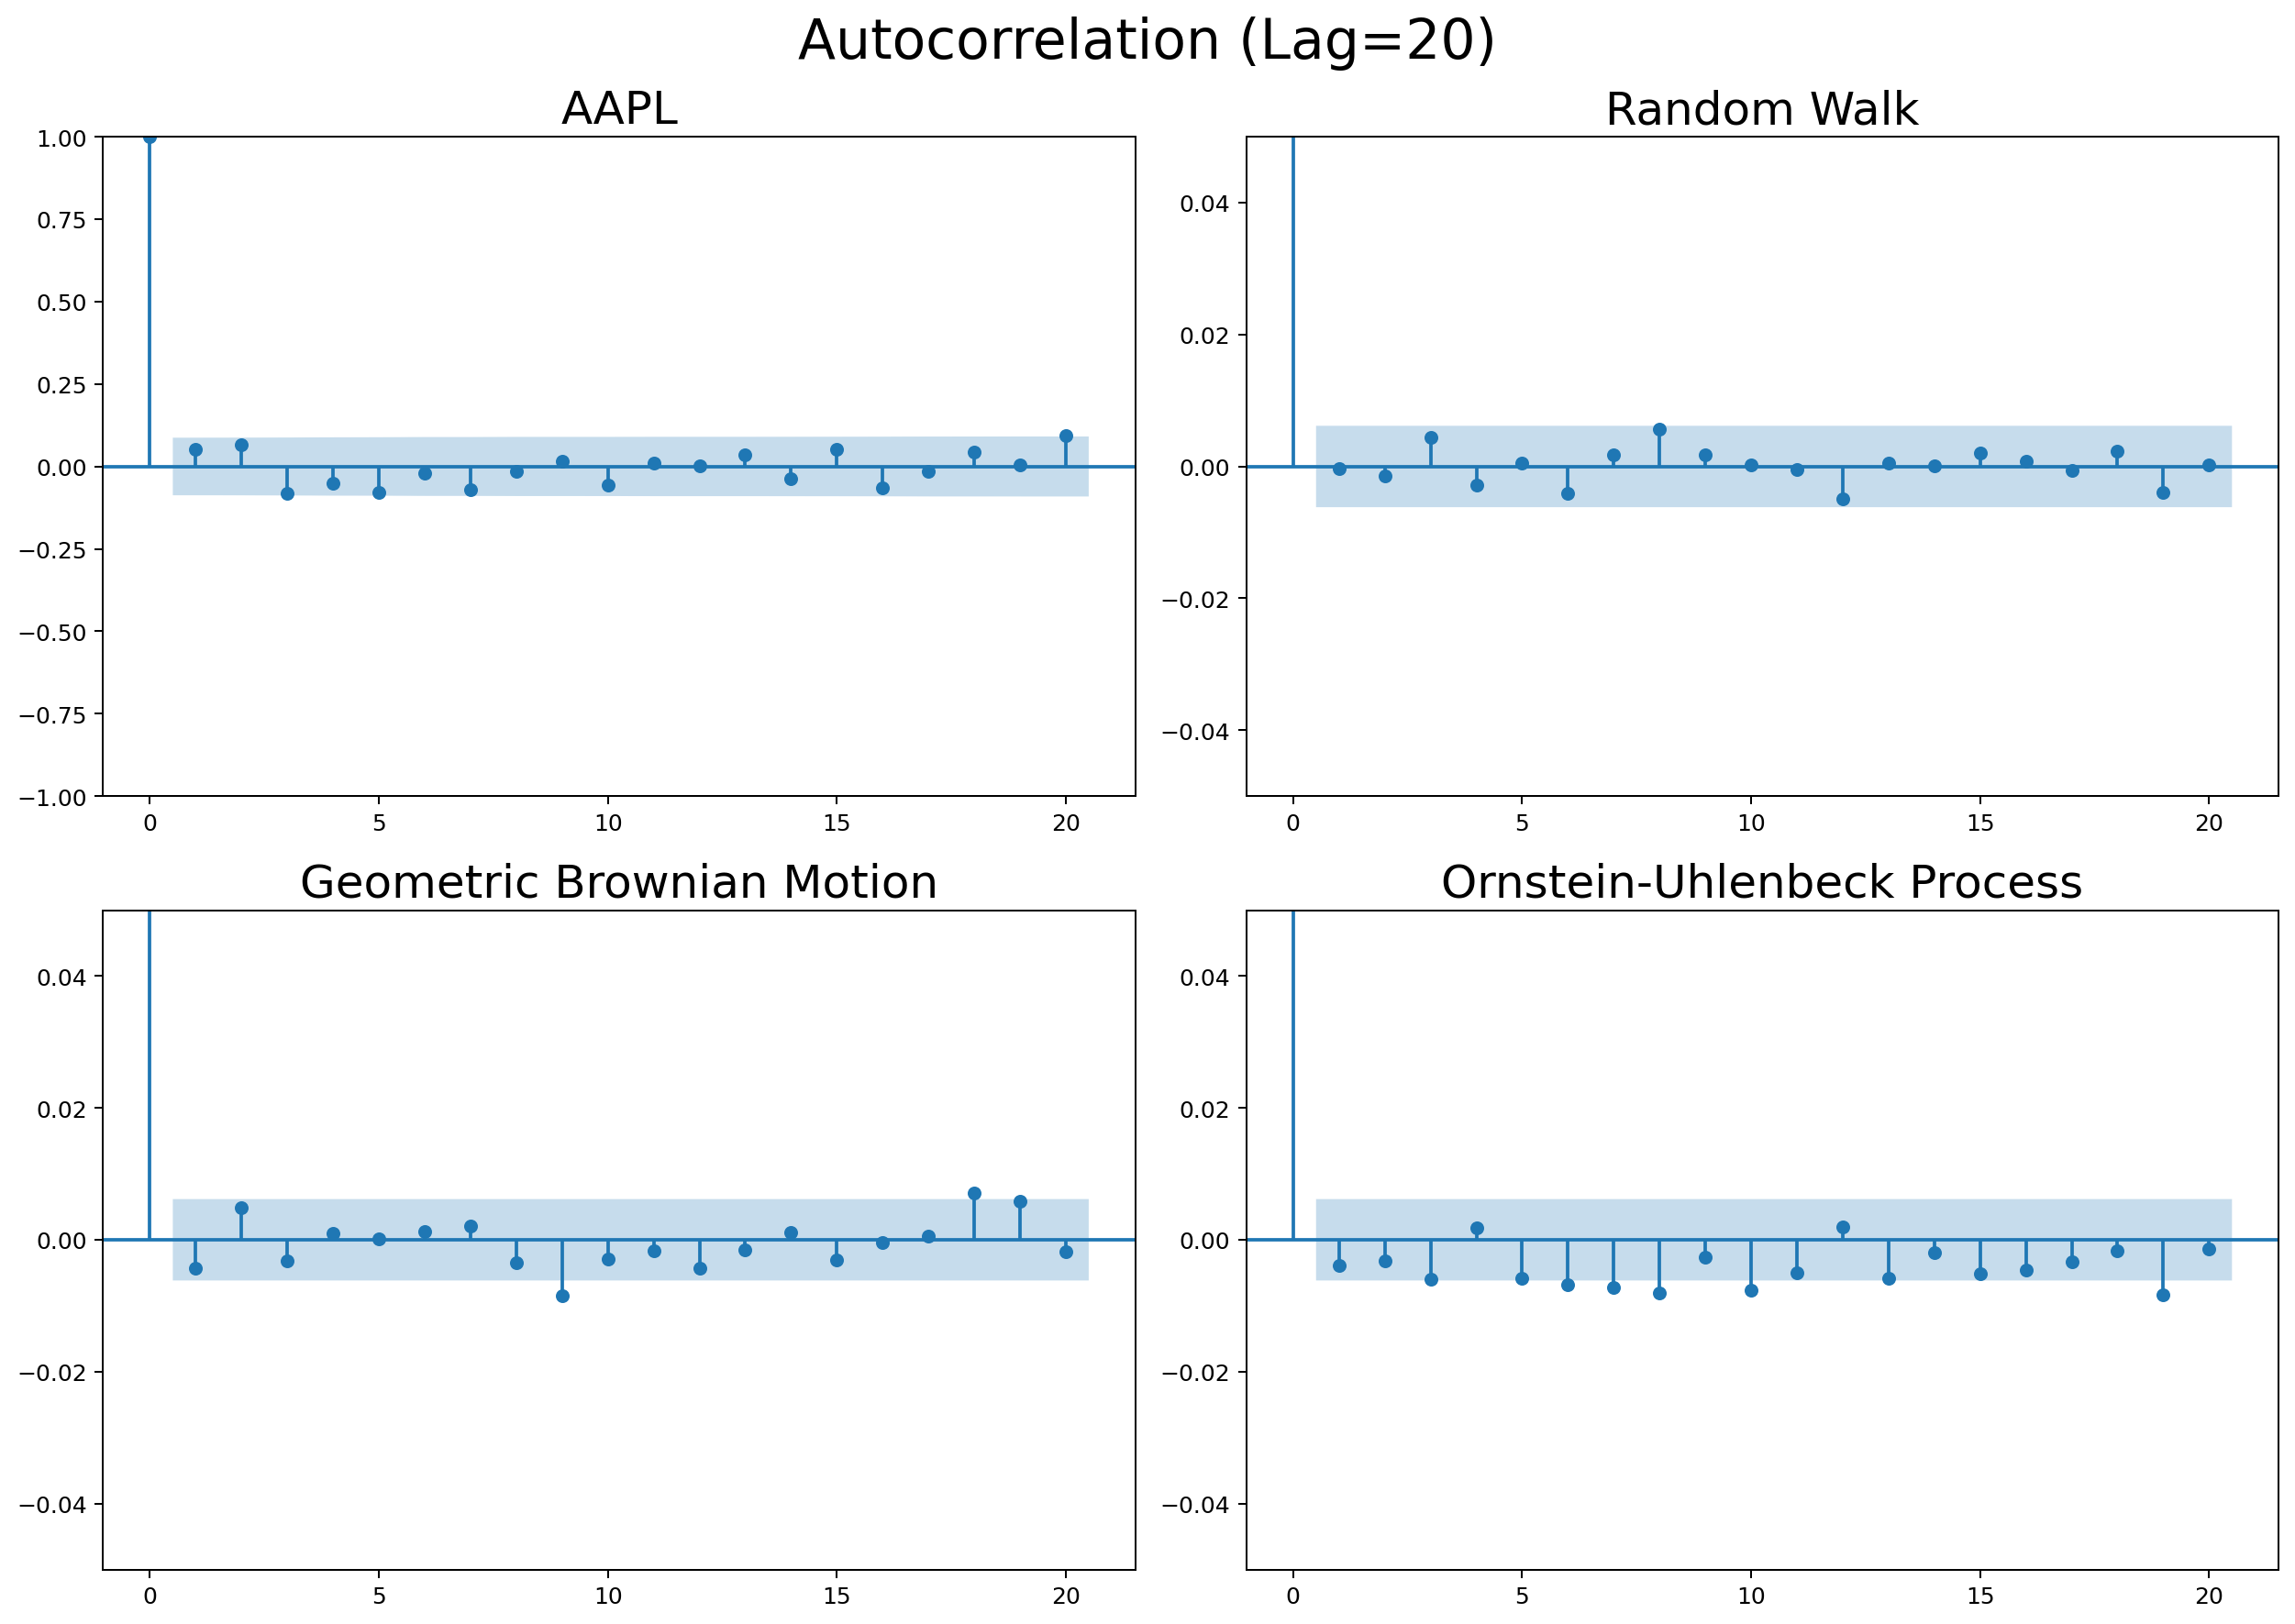
\includegraphics[width=\linewidth,height=0.35\textheight,keepaspectratio]{figures/AAPL/autocorrelation.png}
\caption{AAPL: Log-return autocorrelations; simulated diagnostics pool independent paths.}
\end{figure}
\clearpage
\section{Results: VIX}
\begin{table}[htbp]\centering
\caption{VIX: observed and simulated statistics.}
\resizebox{\linewidth}{!}{\begin{tabular}{lrrrr}\toprule
Metric & VIX & RW & GBM & Log-OU \\
\midrule
Annualized mean log return & 9.10\% & 0.47\% & -80.05\% & 4.68\% \\
Annualized volatility & 141.47\% & 99.74\% & 141.77\% & 141.87\% \\
Return autocorrelation (lag 1) & -0.05712 & -0.0003034 & -0.00425 & -0.006696 \\
ADF p-value: returns & $<10^{-4}$ & $<10^{-4}$ & $<10^{-4}$ & $<10^{-4}$ \\
ADF p-value: price series & 0.0002519 & 0.4088 & 0.3112 & 0.2397 \\
Return skewness & 0.9248 & -0.001577 & -0.005083 & 0.004244 \\
Return kurtosis (Pearson) & 10.11 & 2.994 & 2.973 & 2.997 \\
Maximum drawdown & -74.26\% & -77.41\% & -92.27\% & -83.60\% \\
\bottomrule\end{tabular}}\end{table}
The sample contains 504 observed daily log returns. Its annualized mean log return is 9.10\% and annualized volatility is 141.47\%.

\subsection{Distribution and risk}
Observed Pearson kurtosis is 10.11, versus 2.97--3.00 across the simulated models. Observed skewness is 0.925. Gaussian shocks do not reproduce the observed higher return moments in this run. Observed maximum drawdown is -74.26\%; model drawdowns are path averages and should not be treated as forecasts.

\subsection{Persistence and model fit}
Lag-one return autocorrelation is -0.057. This is a descriptive measure, not a formal test of market efficiency. The ADF test on observed log prices rejects the unit-root null at the 5\% level. That result alone does not identify an OU process. GBM simulated volatility is 141.77\%, while its annualized mean log return is -80.05\%. The drift convention discussed above explains why the mean need not match the data.

\small RW: geometric random walk; GBM: geometric Brownian motion; Log-OU: exponentiated OU process.\normalsize
\clearpage
\subsection*{VIX: Price dynamics}
\begin{figure}[!htbp]\centering
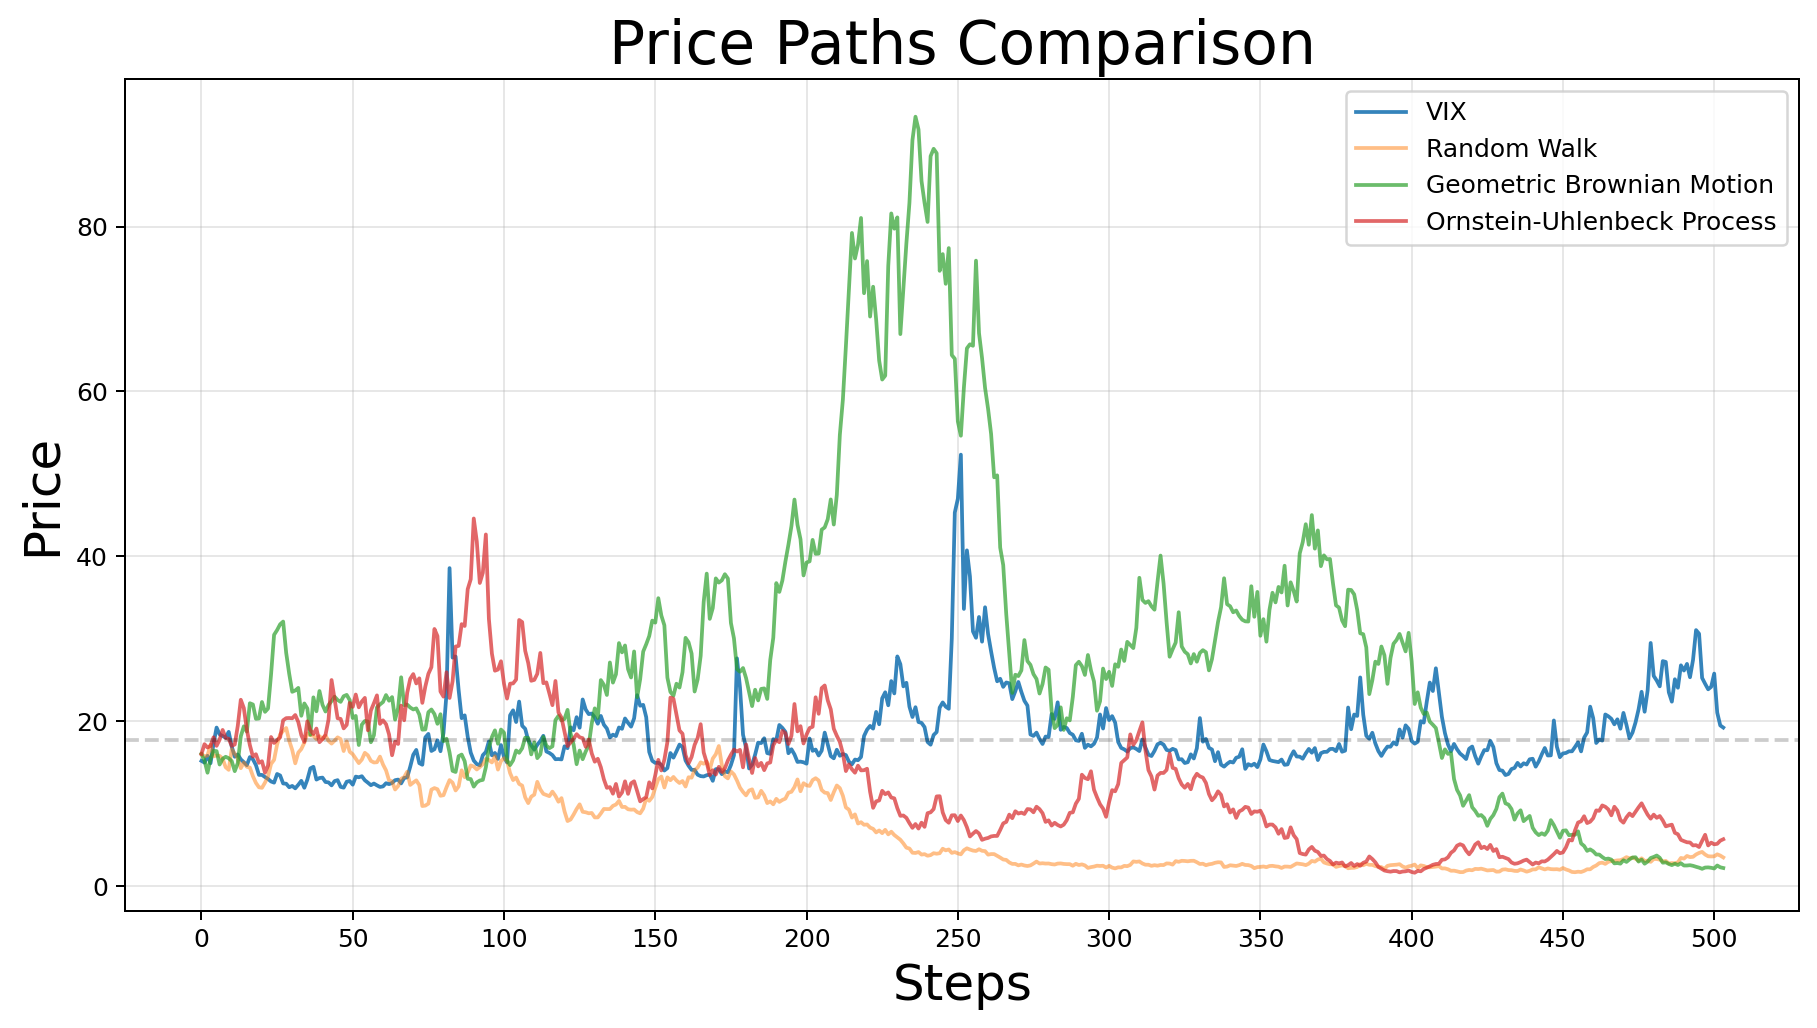
\includegraphics[width=\linewidth,height=0.35\textheight,keepaspectratio]{figures/VIX/price_paths.png}
\caption{VIX: Observed series and one illustrative path per model.}
\end{figure}
\begin{figure}[!htbp]\centering
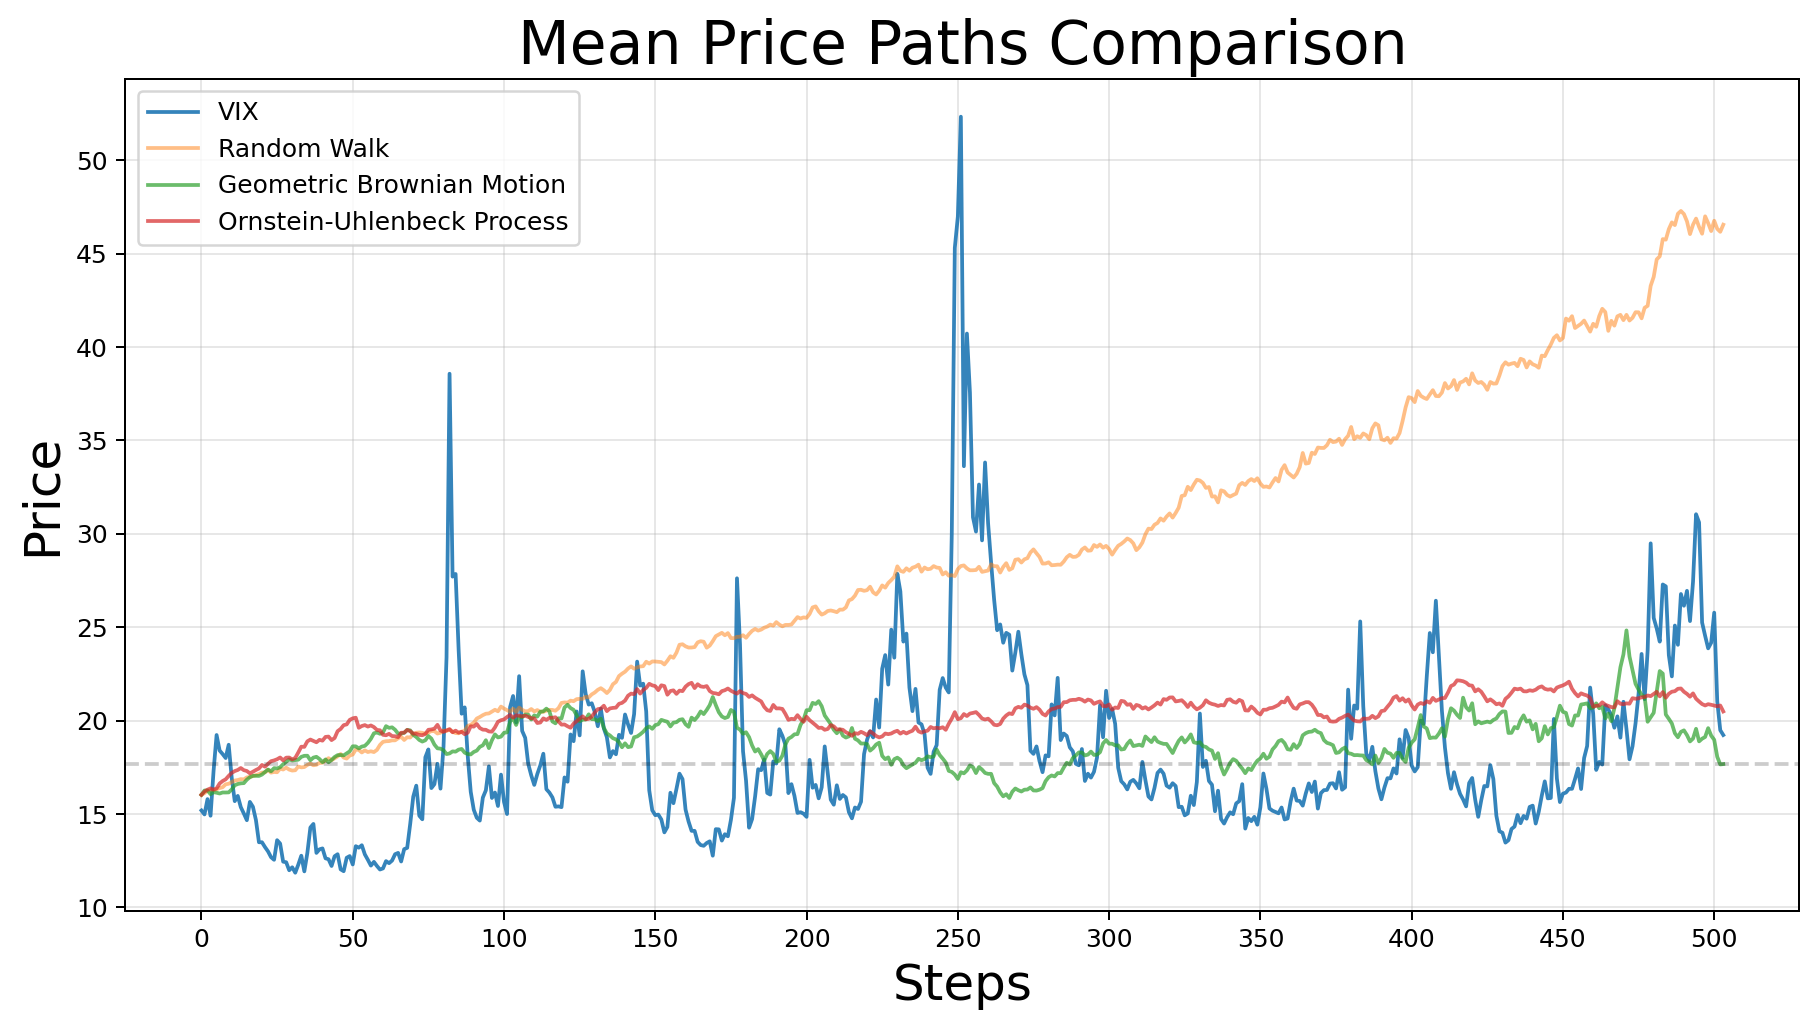
\includegraphics[width=\linewidth,height=0.35\textheight,keepaspectratio]{figures/VIX/mean_paths.png}
\caption{VIX: Observed series and ensemble mean of 200 simulated paths.}
\end{figure}
\clearpage
\subsection*{VIX: Return diagnostics}
\begin{figure}[!htbp]\centering
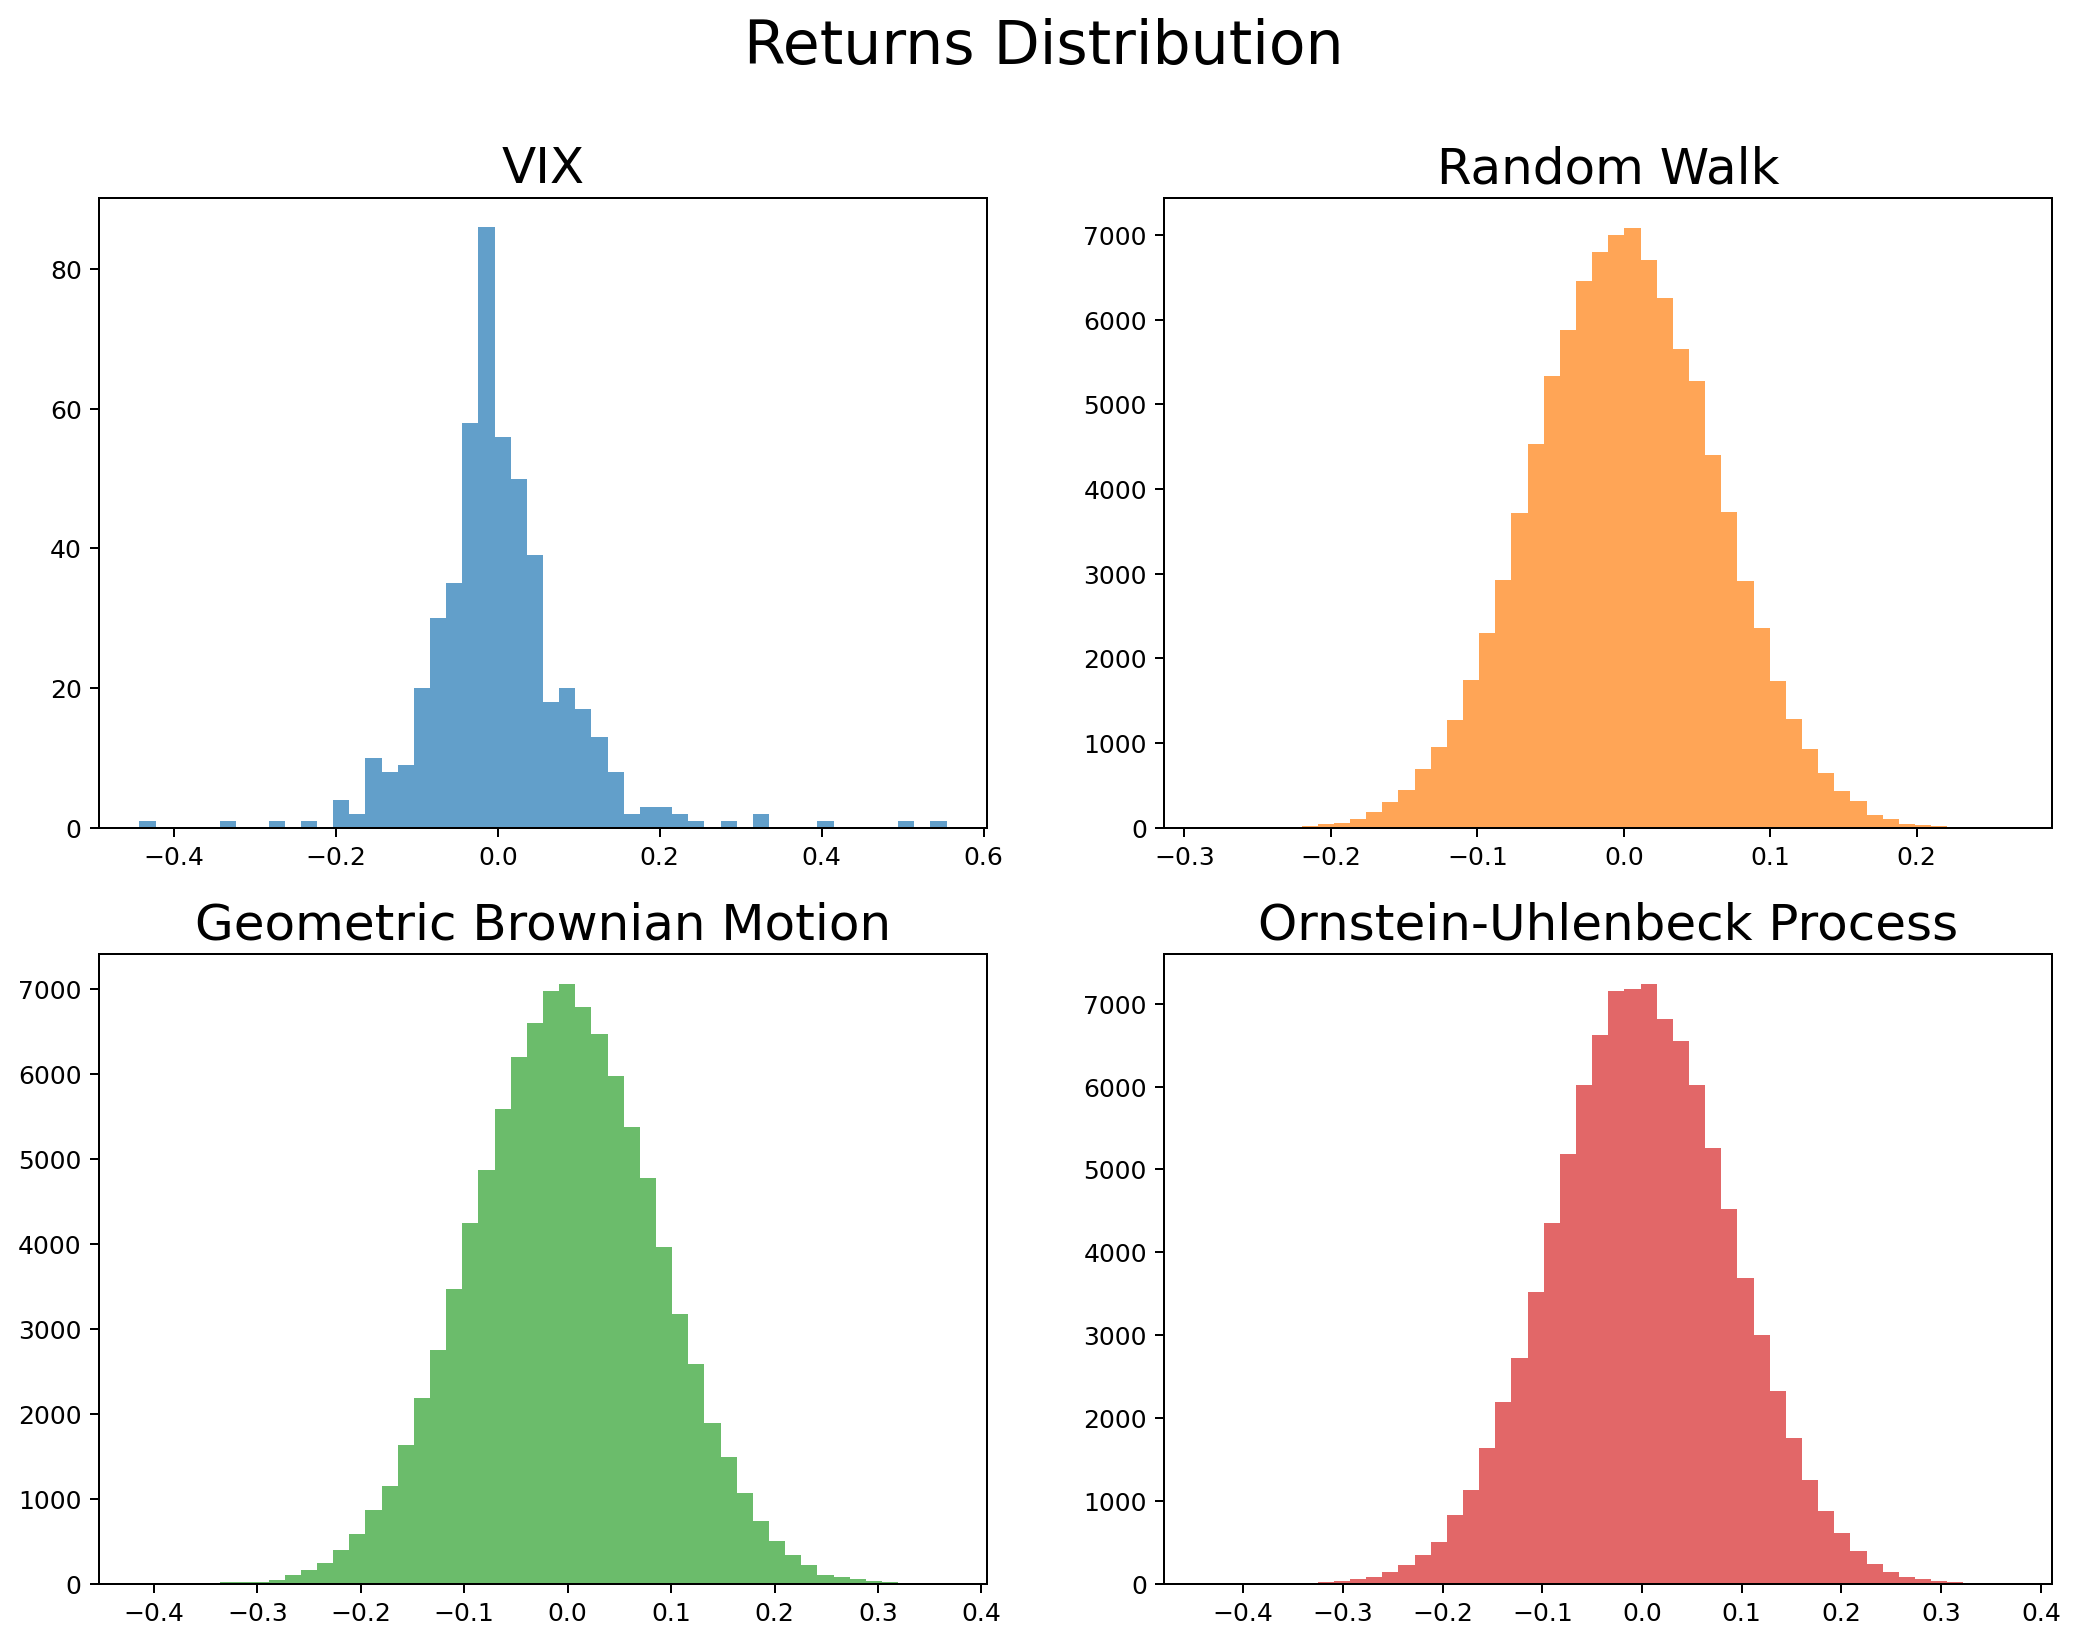
\includegraphics[width=\linewidth,height=0.35\textheight,keepaspectratio]{figures/VIX/distributions.png}
\caption{VIX: Observed and simulated log-return distributions; counts use different sample sizes.}
\end{figure}
\begin{figure}[!htbp]\centering
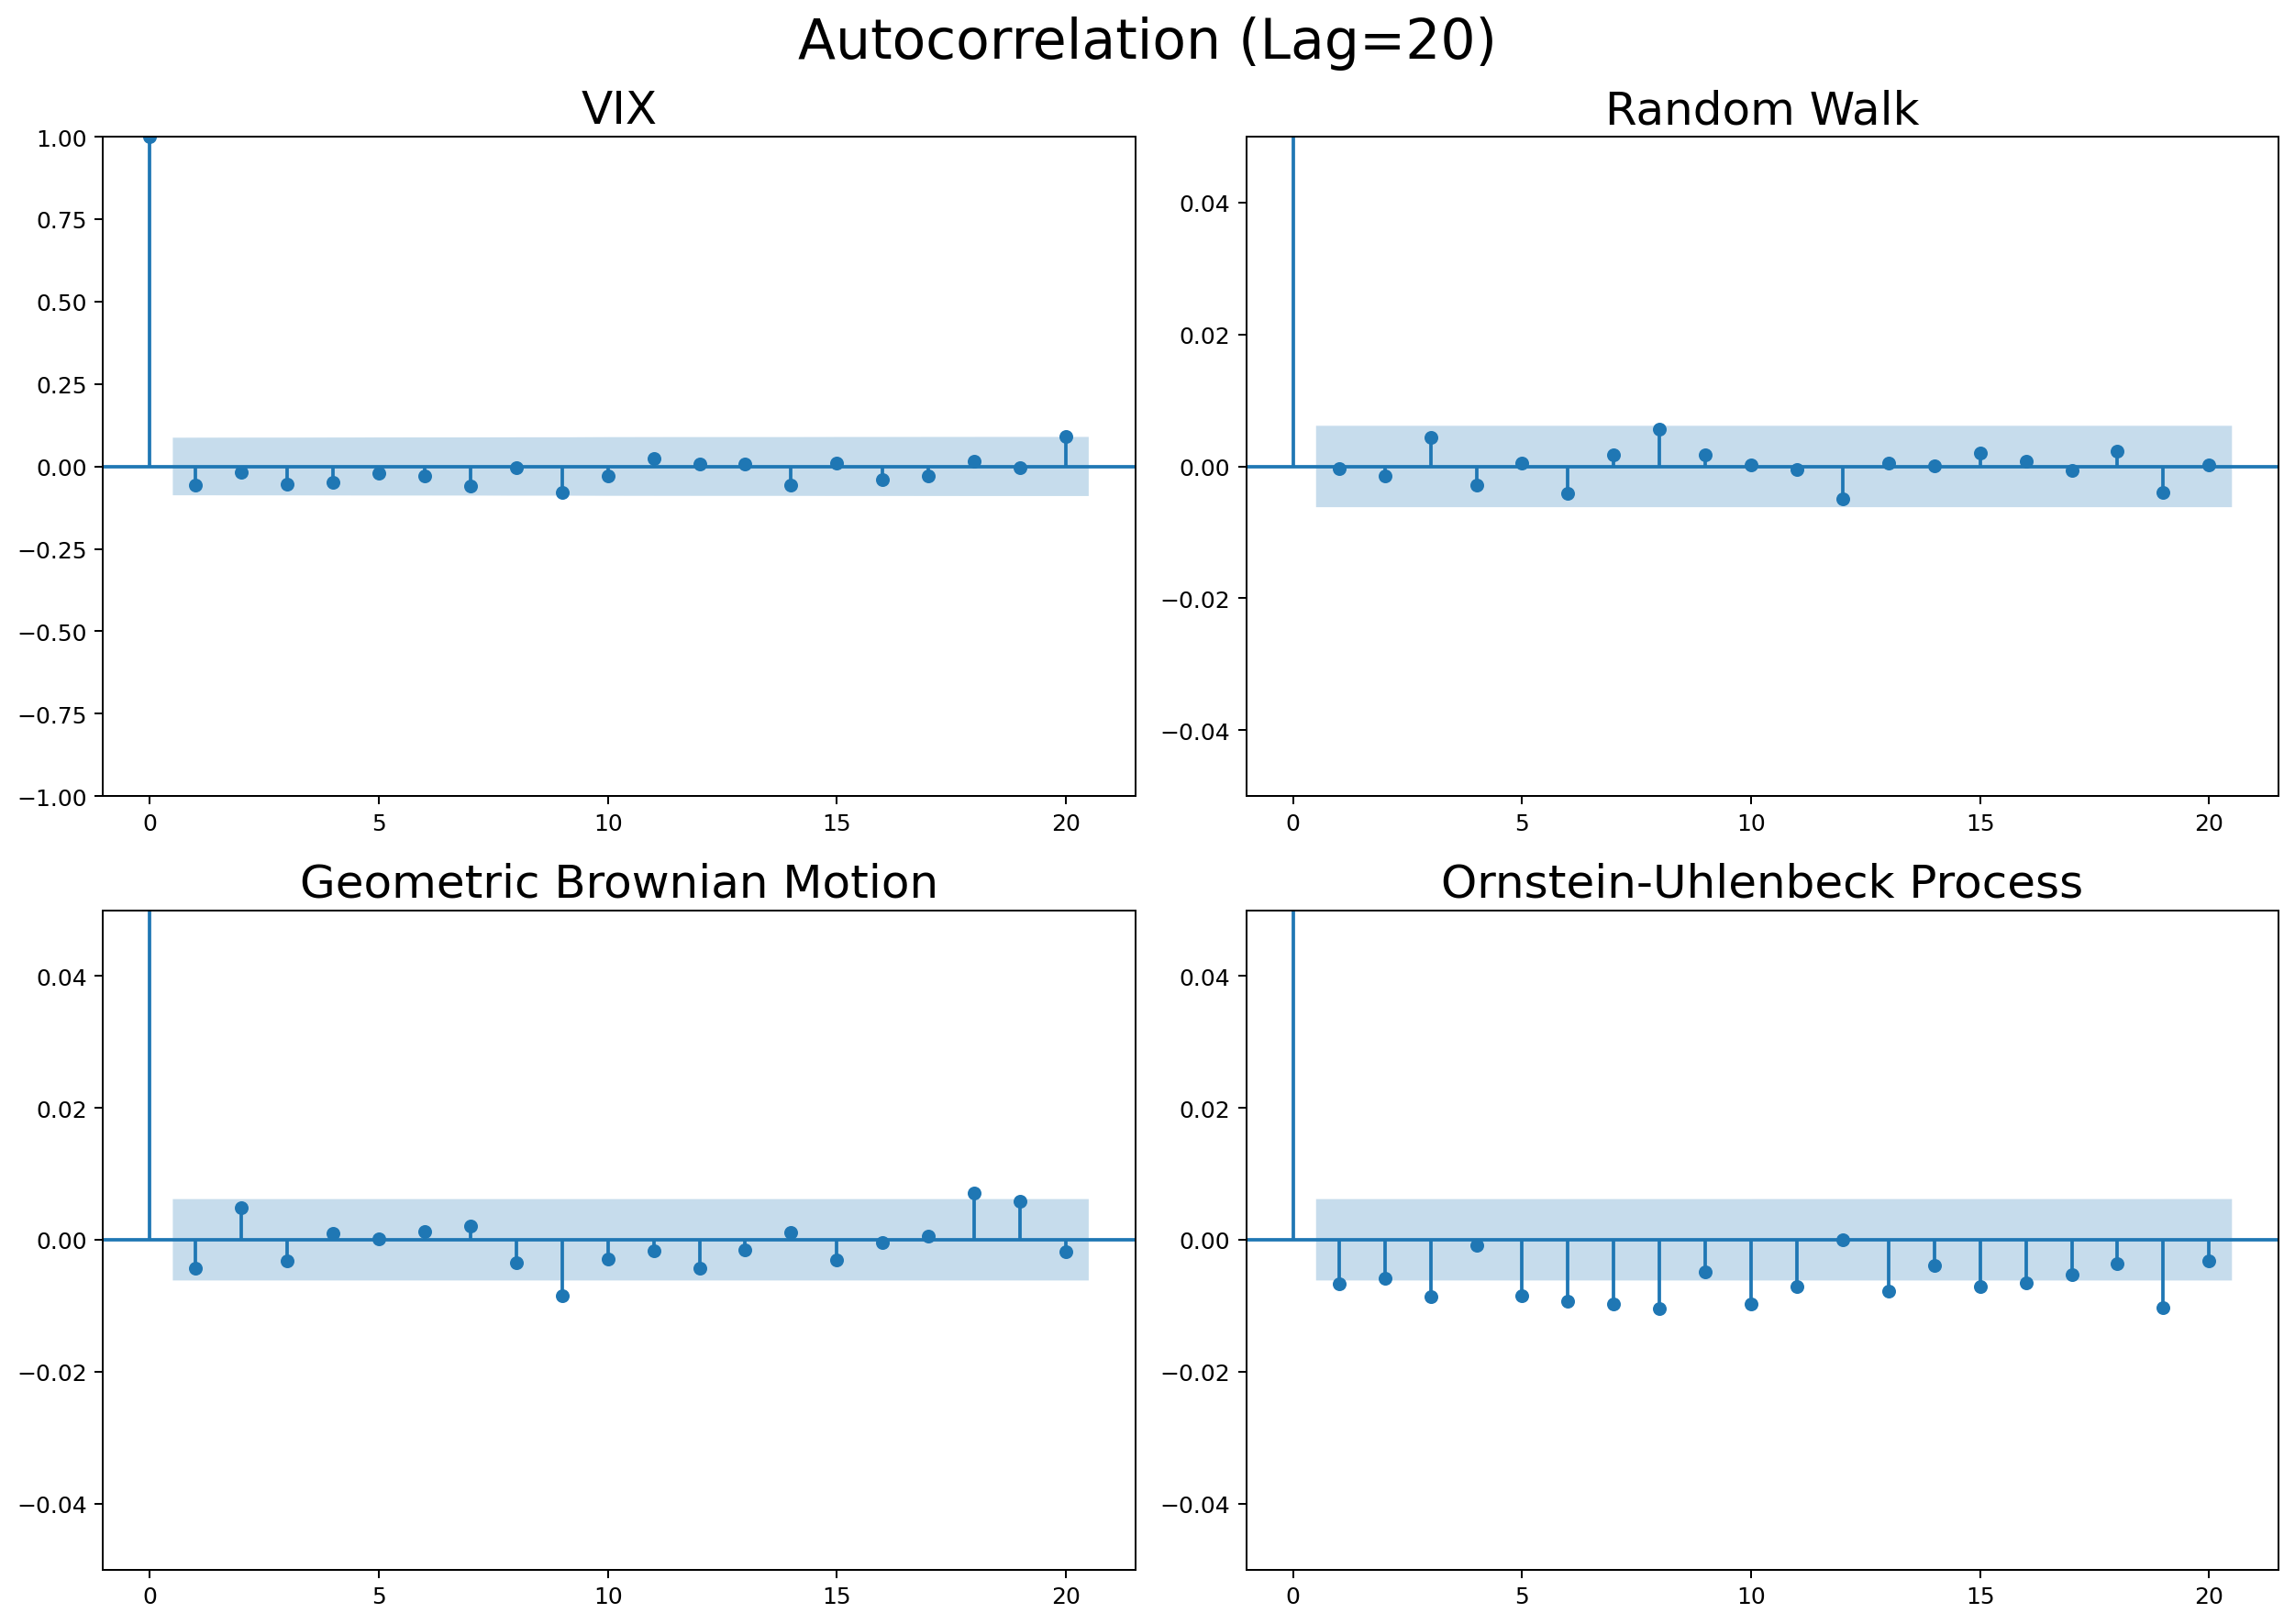
\includegraphics[width=\linewidth,height=0.35\textheight,keepaspectratio]{figures/VIX/autocorrelation.png}
\caption{VIX: Log-return autocorrelations; simulated diagnostics pool independent paths.}
\end{figure}

\clearpage
\section{Discussion and conclusions}
\begin{table}[htbp]\centering
\caption{Observed diagnostics across the two assets.}
\begin{tabular}{lrrr}\toprule
Asset & Return ACF(1) & Pearson kurtosis & Log-price ADF p-value \\\midrule
AAPL & 0.052 & 13.77 & 0.1798 \\
VIX & -0.057 & 10.11 & 0.0002519 \\
\bottomrule\end{tabular}\end{table}

\textbf{H1: Limited evidence on dependence.} The observed autocorrelations
and ACF plots describe serial dependence, but there is no formal joint
whiteness or market-efficiency test in this implementation. The broader
efficiency hypothesis remains unresolved.

\textbf{H2: Limited random-walk fit.} The implemented random walk uses
unit annual log volatility rather than an asset-calibrated scale. Its
risk and distributional fit must therefore be assessed relative to this
specific specification, not as a rejection of every random-walk model.

\textbf{H3: Distributional mismatch.} Both observed series have higher
kurtosis than the approximately Gaussian simulated returns in this run.
GBM reproduces its volatility input closely but does not reproduce these
tail characteristics. Its mean comparison is additionally affected by
the drift convention described in the methodology.

\textbf{H4: Stationarity is not model identification.} The asset-level
ADF results give evidence concerning a unit root under the test's default
specification. Neither rejection nor non-rejection alone establishes
that an OU process is suitable; $\theta$ is not estimated here.

\subsection{Scope and further work}
No single implemented model captures all observed features. The main
lesson is to compare scale, tails, and persistence jointly, rather than
judge models from one illustrative path or a matching volatility.
These results are descriptive, not investment or forecasting evidence.

A stronger follow-up would preserve dated observations, align simulated
and observed price grids, use consistent price transformations for ADF,
compute dependence diagnostics per path, estimate mean-reversion speed,
and evaluate corrected drift calibration on an unseen sample. These are
proposed extensions, not changes made for this report.
\end{document}
